% abstract_takada.tex
% #################################################

\documentclass{article_vdlab_sotsuron_youshi}
\pagestyle{empty}

\usepackage{setspace}
\usepackage{graphicx}
\usepackage{amsmath,amssymb}
\usepackage{comment}
\usepackage{here}

%2段組みの段組み間間隔を設定
\columnsep=1.5cm

\begin{document}
%文字間隔の設定
\kanjiskip = .7pt plus3pt minus 3pt
\xkanjiskip = .7pt plus 3pt minus 3pt
\small
\setstretch{1.1}

%図回りの余白を設定
\setlength{\abovecaptionskip}{0mm}
\setlength{\belowcaptionskip}{0mm}
\setlength{\floatsep}{0mm}
\setlength{\textfloatsep}{0mm}
\setlength{\intextsep}{3mm}
\setlength{\dblfloatsep}{0mm}
\setlength{\dbltextfloatsep}{0mm}

% #################################################

\twocolumn[
  \begin{center}
    % 論文題目と氏名
    \jtitle{IDCS制御手法を用いたHILSシステムの検討}
    \jauthors{中川 夏}
    \etitle{Investigation of HILS system using IDCS}
    \eauthors{Natsu Nakagawa}
  \end{center}
]

%文字間隔の設定
\kanjiskip = .7pt plus3pt minus 3pt
\xkanjiskip = .7pt plus 3pt minus 3pt
\small
\setstretch{1.1}

% #################################################
\section{緒言}
HILSとは,Hardware-in-the-Loop Simulationの略称であり,対象のハードウェアをシミュレーションループ内に直接組み込むことで特性評価を行うシステムである.自動車のタイヤ―サスペンション系には非線形特性を有したダンパがあるためシミュレーションで評価するのは難しく,実写走行試験による評価では,天候等の影響により同一条件下での繰り返し試験を行うことが難しい.これらの問題を解決するシステムとしてHILSシステムが用いられている\cite{hils}.HILSシステムはハードウェアの計測結果を用いて解析をし,その解析結果に基づいてアクチュエータへの入力値を決定する.

本研究では,自動車のタイヤ―サスペンション系の上下動を再現するHILSシステムを対象とし,アクチュエータの制御手法を検討し,HILSシステムの再現性の向上を図る.制御手法にはIDCS制御手法を用いた.ハードウェアの挙動と解析結果を比較することで,検討した制御手法におけるHILSシステムの再現性の影響を評価した.

\vspace{4mm}
\section{HILSシステム}
本研究で使用するHILSシステムの概要を図\ref{fig:HILS}に示す.このHILSシステムは自動車のタイヤ―サスペンション系の上下動を試験機で再現するシステムである.HILSシステムの構成は,車両運動解析や解析結果に基づいてアクチュエータへの入力を決定するソフトウェア部と,試験装置のハードウェア部からなる.本システムでは試験装置のばね上-ばね下相対変位が解析結果とが一致するようにアクチュエータの入力値を決定する.解析モデルには上下2自由度振動系を用い,計測されたダンパの減衰力を用いて解析を行う.試験装置の路面下部にはアクチュエータであるモータが取り付けられており,その解析結果に基づいて入力値が決定されるため,上下挙動の再現が可能である.

\vspace*{5mm}
\begin{figure}[H]
  \begin{center}
    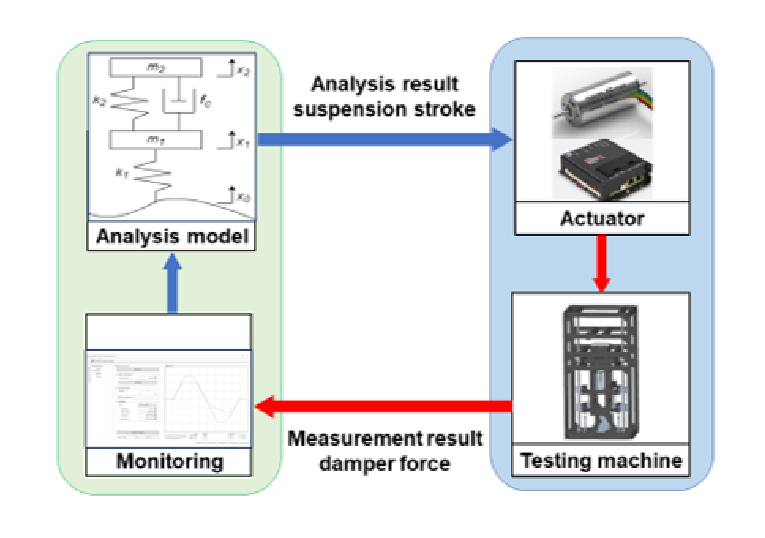
\includegraphics[height=60mm]{figure/HILS_loop.eps}
    \vspace*{2mm}
    \caption{System overview of Tire-Suspension HILS system}
    \label{fig:HILS}
  \end{center}
\end{figure}

\newpage
ハードウェア部で用いるHILS試験機を図\ref{fig:testing_machine}に示す.この装置は上下1自由度で,タイヤ―サスペンション系をばね下,ばね,ダンパで表している.路面部にアクチュエータを取り付けており,アクチュエータの入力$\bar{x}_0$はソフトウェア部の解析結果に基づいて決定する.解析モデルと装置ではシステムの自由度が異なるため,入力$\bar{x}_0$に対する試験機のばね上ばね下間変位$-\bar{x}_1$で解析モデルのサスペンションストロークを再現している.ばね上ばね下間変位,ダンパ力はレーザ変位計,ロードセルを用いて計測している.

\vspace{5mm}
\begin{figure}[H]
 \centering
 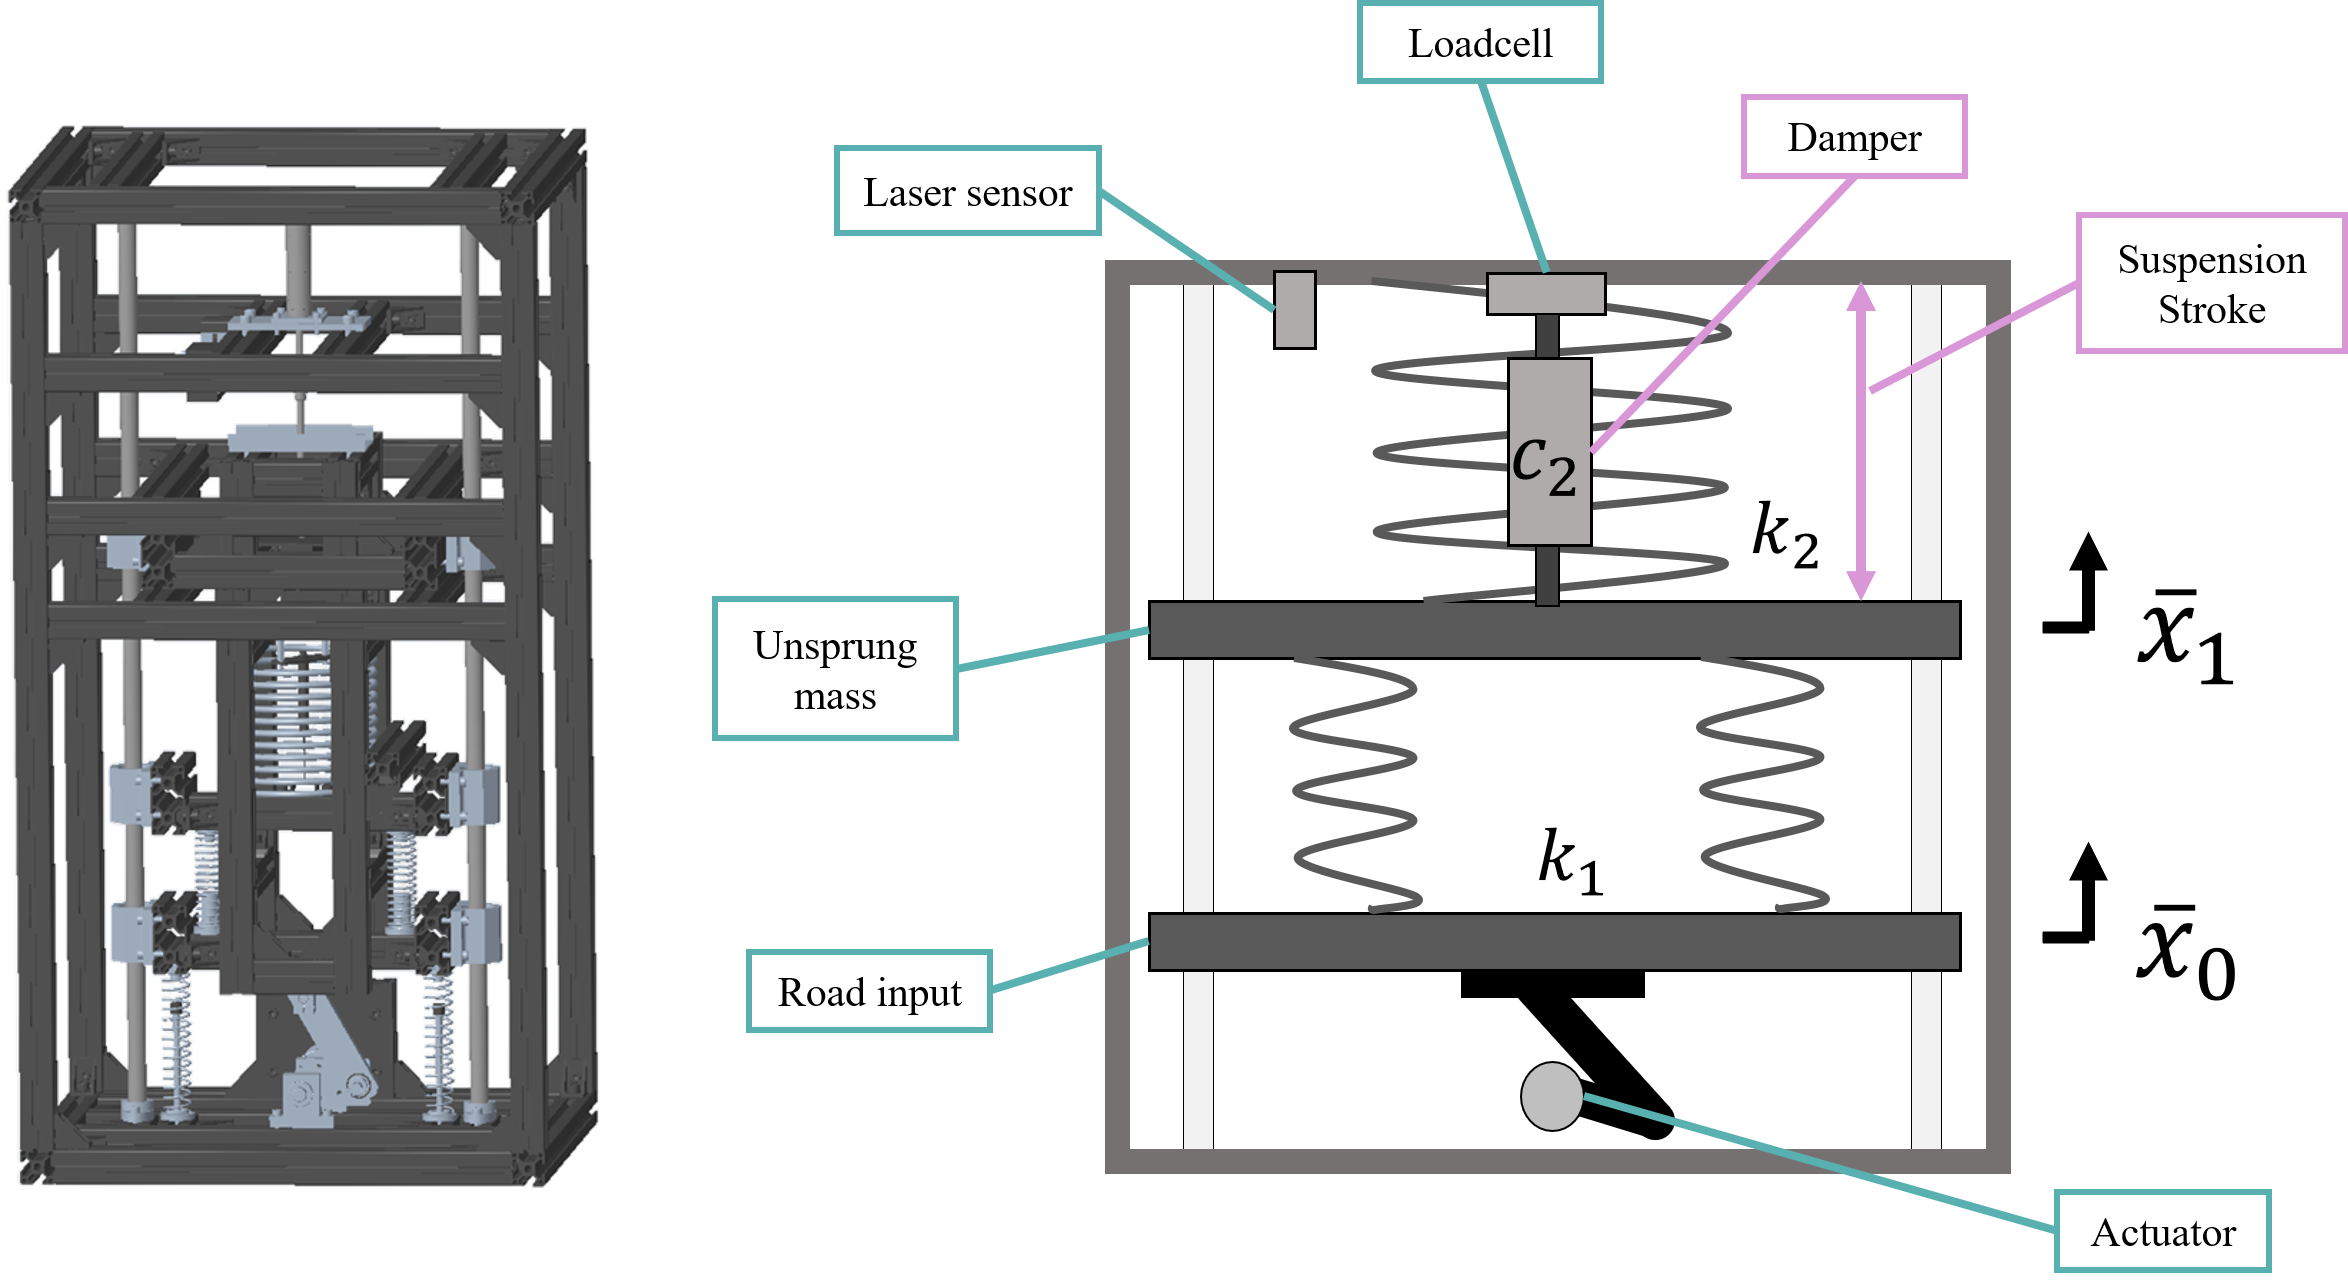
\includegraphics[height=50mm]{figure/HILS_machine.eps}
 \vspace{-5mm}
  \caption{HILS testing machine}
 \label{fig:testing_machine}
\end{figure}

\vspace*{5mm}
解析モデルに用いた上下2自由度モデルは,車両の上下動を表すことのできるモデルである.\cite{2dof}.上下2自由度モデルを図\ref{fig:analysis_model}に,モデルの諸元を表\ref{tab:analysis_parameter}に示す.また,このモデルの運動方程式は以下の通りである.

\noindent
\begin{eqnarray}
 \label{eq:2dof_m1} &&m_1\ddot x_1 + k_1(x_1-x_0) + k_2(x_1-x_2) - f_c = 0\\
 \label{eq:2dof_m2} &&m_2\ddot x_2 + k_2(x_2-x_1) + f_c = 0
\end{eqnarray}

ここで,$m_1$はばね下質量 ,$m_2$はばね上質量,$k_1$,$k_2$はばね定数,$f_c$はダンパ力,$x_0$は路面変位,$x_1$はばね下変位,$x_2$はばね上変位である.この解析モデルを用いて路面変位$x_0$に対するサスペンションストローク$x_2-x_1$を計算し,HILS試験機で再現する.

\begin{figure}[H]
  \begin{minipage}{0.5\hsize}
    \begin{center}
      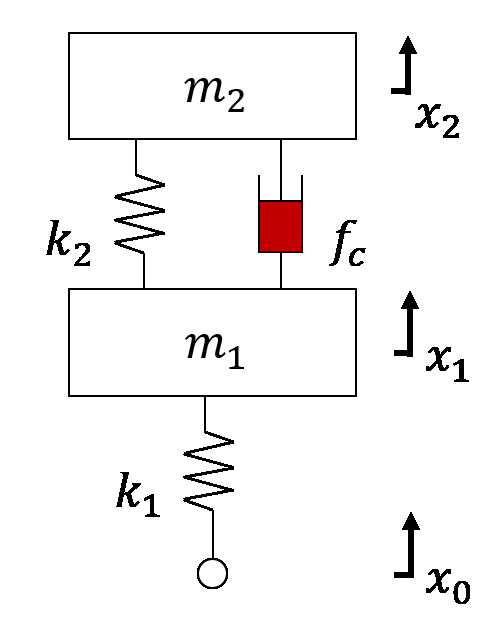
\includegraphics[height=35mm]{figure/analysis_model.eps}
      \caption{Analysi model}
    \label{fig:analysis_model}
    \end{center}
  \end{minipage}
  \begin{minipage}{0.45\hsize}
      \begin{center}
	\makeatletter
	\def\@captype{table}
	\makeatother
	\caption{Parameter}
	\label{tab:analysis_parameter}
	  \begin{tabular}{cc}\hline
	    $m_1$ [kg] & 1.3\\
	    $m_2$ [kg] & 6.9\\
	    $k_1$ [N/m] & 2200\\
	    $k_2$ [N/m] & 439\\\hline
	  \end{tabular}
      \end{center}
  \end{minipage}
\end{figure}

\newpage
\section{IDCS制御手法}
Inverse Dynamics Compensation via 'Simulation of feedback control system'(IDCS)制御手法はシステムの順動力学を用いたフィードバック制御シミュレーションにより近似的な逆動力学の計算を行う手法である\cite{method_idcs}.図~\ref{fig:idcs_block}にIDCS制御手法のブロック線図を示す.点線で囲まれた部分は数値シミュレーション環境であり,$P_m$は試験機$P$を模擬したモデルである.制御器$K$と$P_m$で構築されるフィードバック制御系はシミュレーション上では理想的な制御を行えるため,$P_m$の出力$y_m$は目標値$r$に追従する.ここで$P_m$と$P$が同一であると考えると,$P$の出力$y$は目標値$r$に追従する.

\vspace*{2mm}
\begin{figure}[htp]
  \begin{center}
    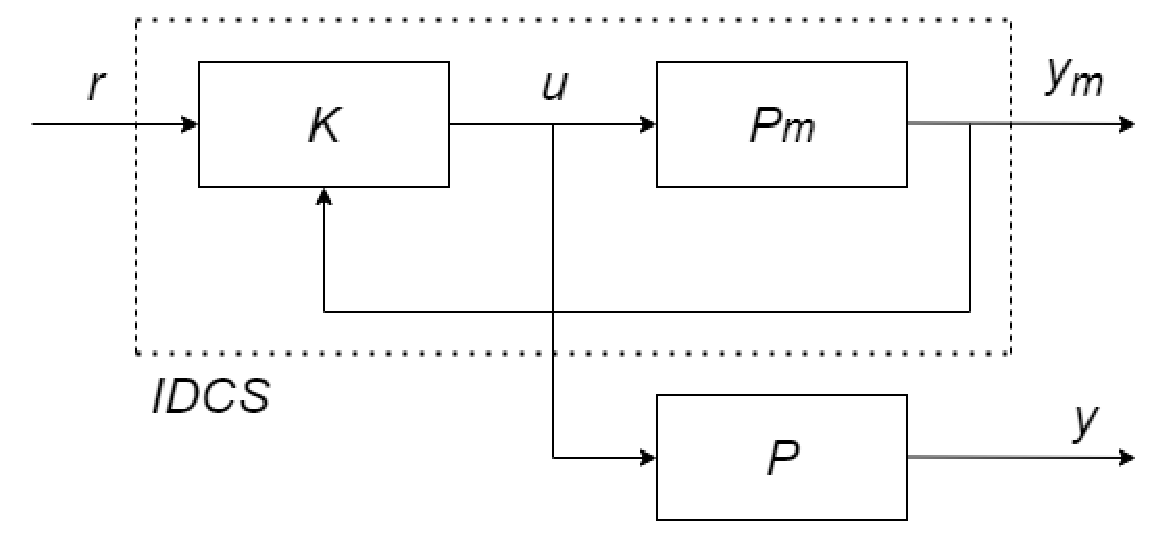
\includegraphics[height=30mm]{figure/idcs_block.eps}
    \vspace*{1mm}
    \caption{Block diagram(IDCS)}
    \label{fig:idcs_block}
  \end{center}
\end{figure}

IDCS制御系を組み込んだHILSシステムを図~\ref{fig:idcs_diagram}に示す.ハードウェアモデルは試験機を模擬したモデルである.本研究で用いるIDCS制御系内の制御器$K$は,目標値とハードウェアモデルのサスペンションストローク$-\bar{x_1}$の偏差を取り,比例ゲイン$K_p$を用いてアクチュエータへの入力を決定している.本研究で用いるハードウェアモデルでは線形・非線形のダンパモデルを使用し,比較する.

\vspace*{3mm}
\begin{figure}[htp]
  \begin{center}
    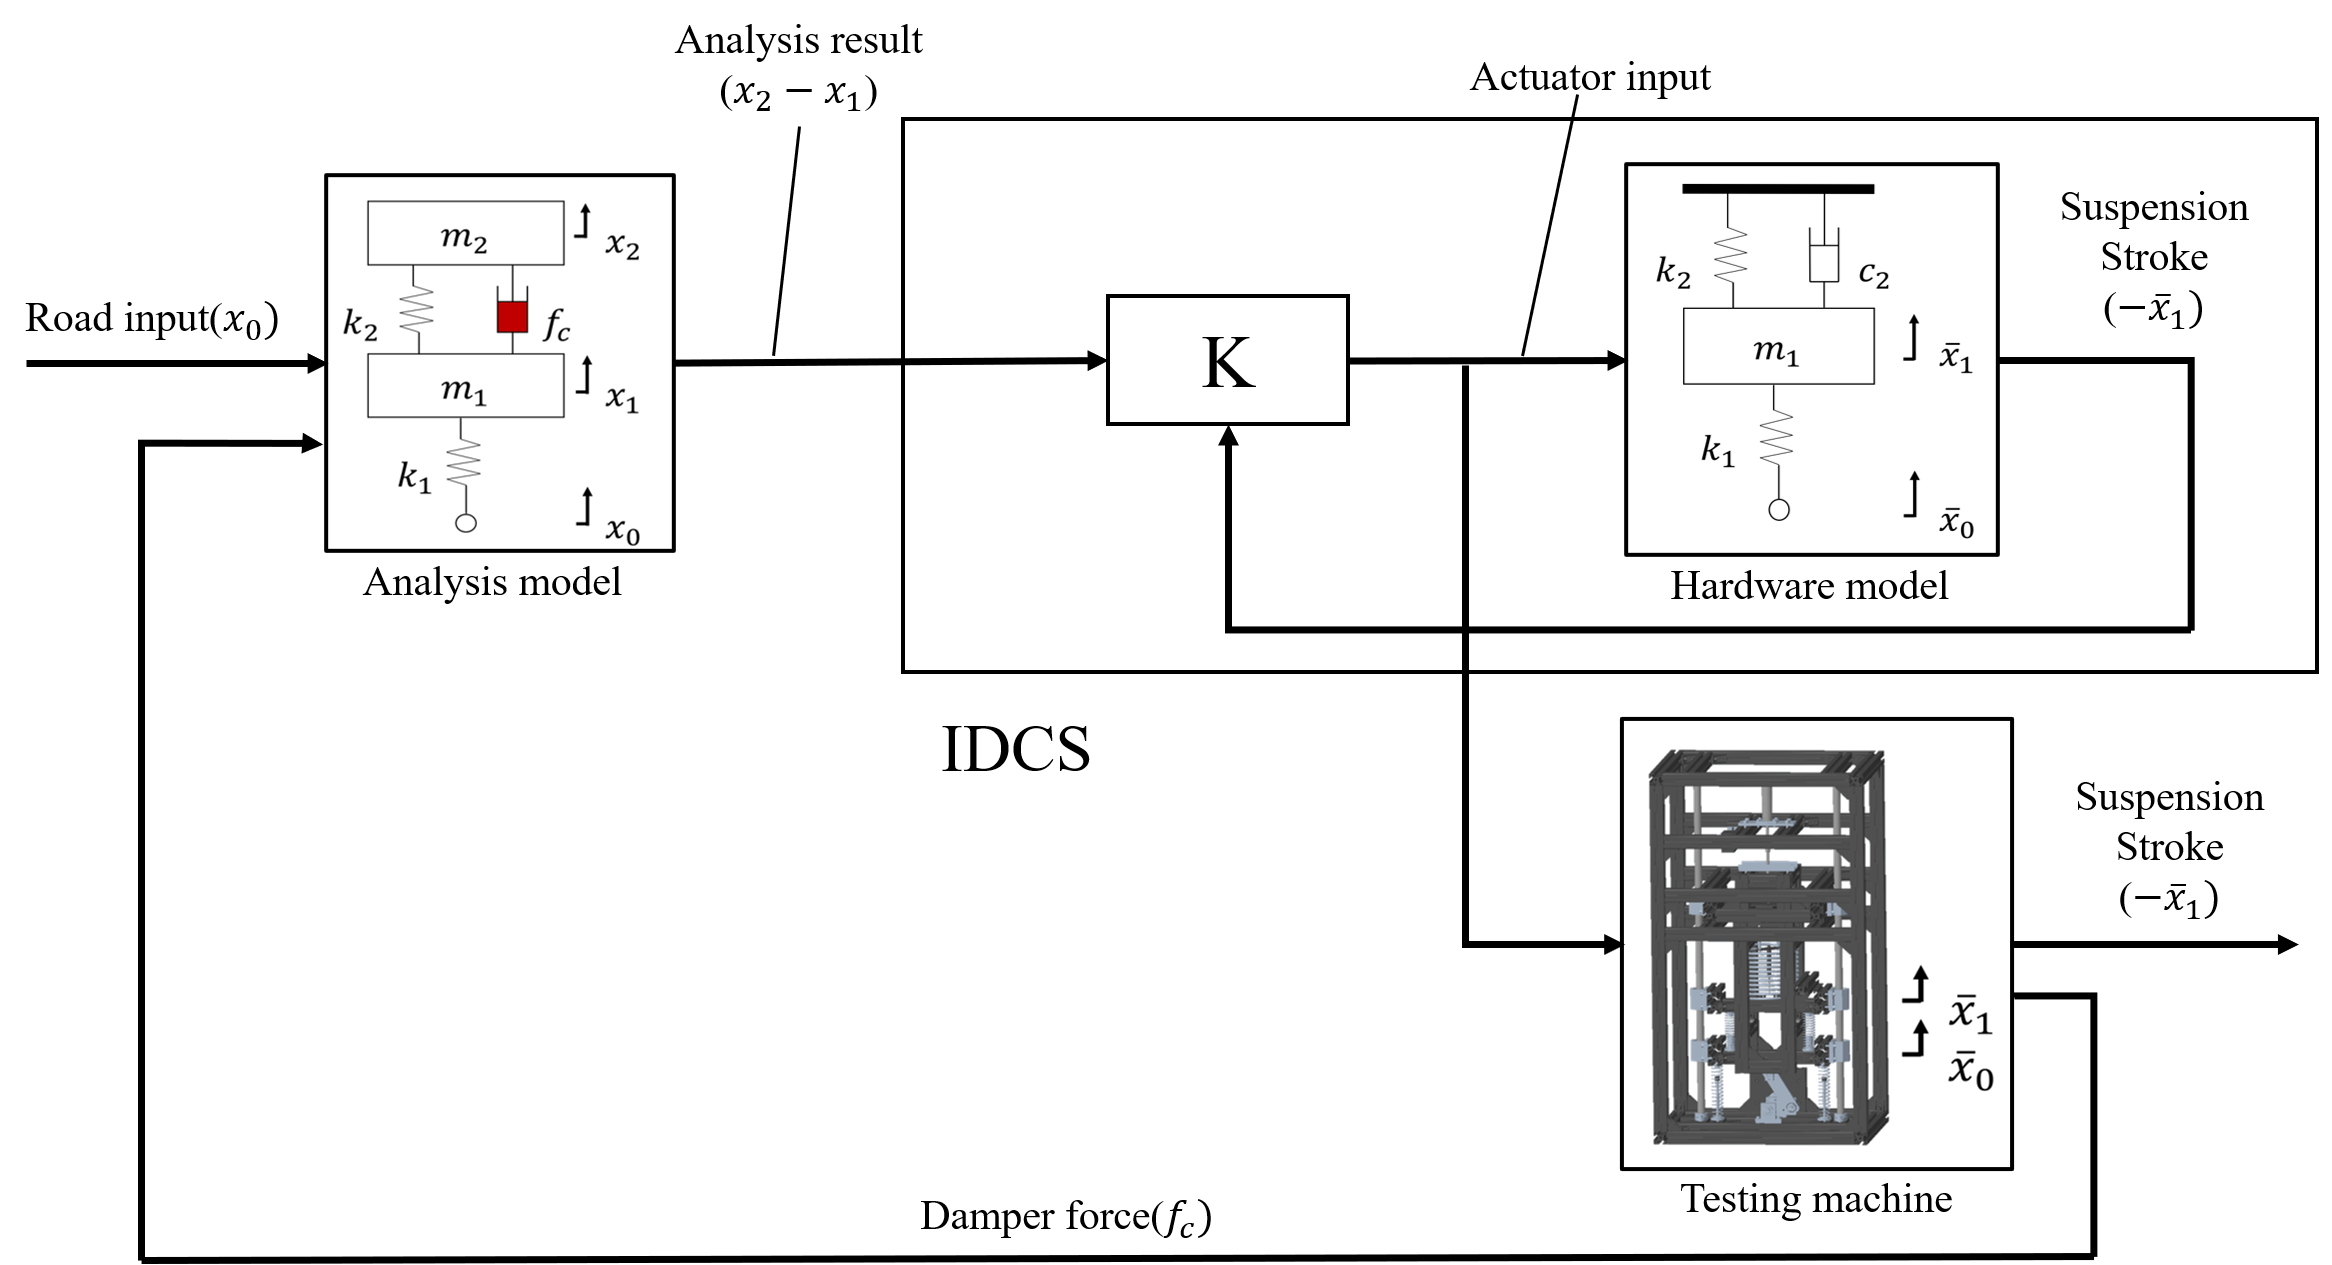
\includegraphics[height=45mm]{figure/idcs_diagram.eps}
    \vspace*{1mm}
    \caption{Block diagram of HILS system(IDCS)}
    \label{fig:idcs_diagram}
  \end{center}
\end{figure}

\section{非線形ダンパモデル}
IDCSを用いた制御において,制御精度を高めるには制御対象と制御対象とのモデル化誤差を小さくする必要がある.そこで本研究で使用するダンパの単体試験を行い,試験データより作成した非線形性を考慮したダンパモデルを試験機モデルに組み込む.作成したダンパモデルに周波数1Hz,振幅を変化させた時のF-X線図,F-V線図を図~\ref{fig:damper}に示す.

\vspace*{3mm}
\begin{figure}[h]
  \begin{tabular}{cc}
  \begin{minipage}{0.5\hsize}
  \begin{center}
    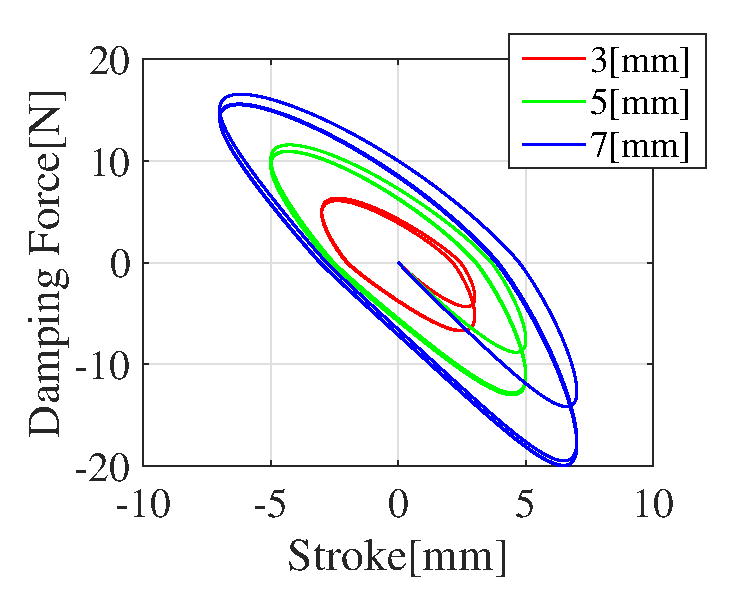
\includegraphics[height=30mm]{figure/damper_fx.eps}
    \end{center}
    \begin{center}
      \vspace{-3mm}
    \ F-X\
    \end{center}
  \end{minipage}
  \begin{minipage}{0.5\hsize}
     \begin{center}
      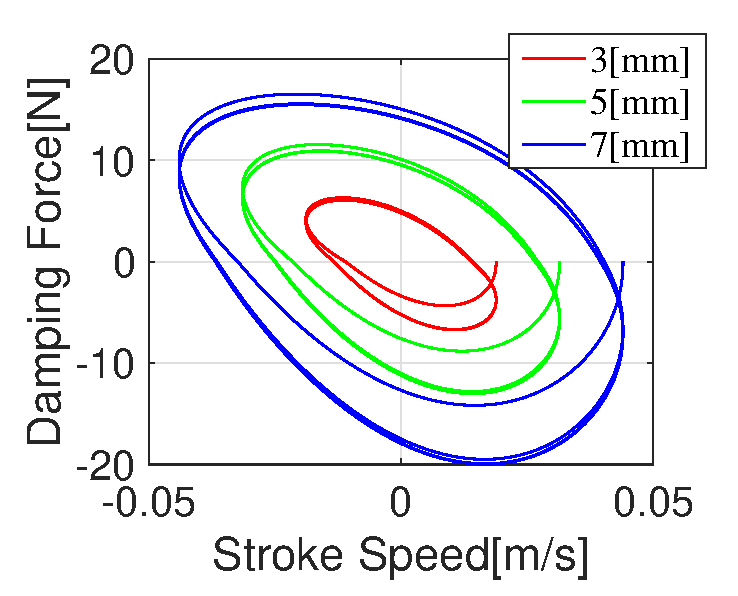
\includegraphics[height=30mm]{figure/damper_fv.eps}
      \end{center}
      \begin{center}
        \vspace{-3mm}
      \ F-V\
    \end{center}
  \end{minipage}
  \end{tabular}
  \caption{Difference in amplitude(Frequency:1Hz)}
    \label{fig:damper}
\end{figure}

\newpage
\section{HILS試験}
% --------- メモ
% 線形・非線形ダンパを用いたIDCSがちゃんと追従していることを示して,非線形性を考慮した制御が可能であることを示す.

IDCS制御手法を用いたHILSシステムの再現性の評価を行う.試験機モデルに線形ダンパを組み込んだ場合について,周波数3Hz,振幅5mmの正弦波の路面入力試験の試験結果を図~\ref{fig:idcs_linear}に示す.この時の制御器の比例ゲイン$K_p$は15である.(a)は解析モデルの計算結果とレーザ変位計による計測結果であり,(b)はIDCS制御系内の試験機モデルの計算結果とレーザ変位計による計測結果を示す.

図~\ref{fig:idcs_linear}より試験機の計測結果と解析結果,試験機の計測結果と試験機モデルの計算結果が同じ挙動を示していることがわかる.

\vspace*{3mm}
\begin{figure}[h]
  \begin{tabular}{cc}
  \begin{minipage}[t]{0.5\hsize}
  \begin{center}
    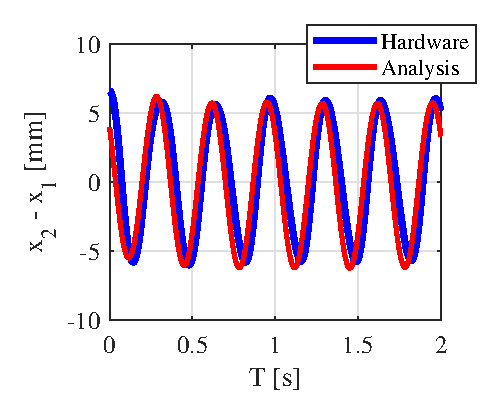
\includegraphics[height=30mm]{figure/sus_linear_5_3.eps}
    \end{center}
    \begin{center}
      \vspace{-3mm}
    \ (a)Comparison with Analysis\
    \end{center}
  \end{minipage}
  \begin{minipage}[t]{0.5\hsize}
     \begin{center}
      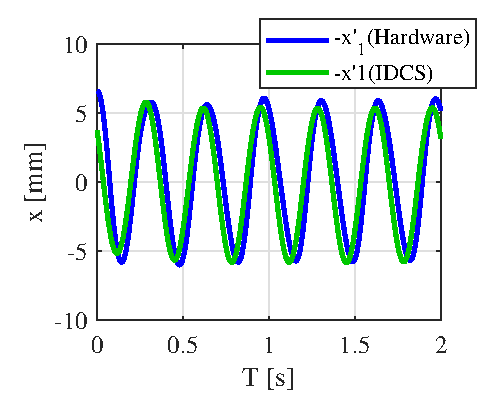
\includegraphics[height=30mm]{figure/idcs_linear_5_3.eps}
      \end{center}
      \begin{center}
        \vspace{-3mm}
      \ (b)Comparison with Hardware model\
    \end{center}
  \end{minipage}
  \end{tabular}
  \caption{Result(linear damper)}
    \label{fig:idcs_linear}
\end{figure}

非線形ダンパモデルを組み込んだIDCS制御系を用いた制御手法において,上記試験と同様の試験を行ったときの試験結果を図~\ref{fig:idcs_nonlinear}に示す.この時の比例ゲイン$K_p$は7である.

比例ゲインの値が線形ダンパを組み込んだ時よりも小さくなるのは,非線形ダンパモデルを組み込んだことで,ソフトウェア部の計算量が多くなり,ステップ時間が大きくなったことが原因である.ゲインは低くなったが,試験機の出力値が目標値である解析結果に追従していることが確認できる.

\vspace*{2mm}
\begin{figure}[h]
  \begin{tabular}{cc}
  \begin{minipage}[t]{0.5\hsize}
  \begin{center}
    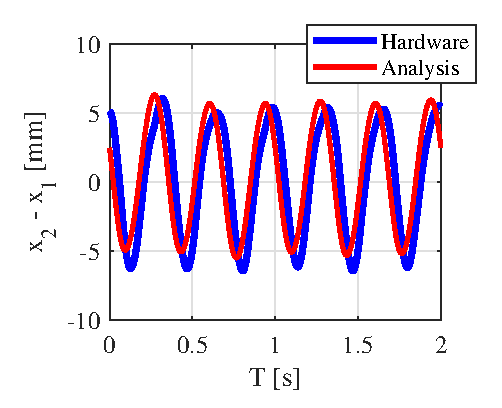
\includegraphics[height=30mm]{figure/sus_nonlinear_5_3.eps}
    \end{center}
    \begin{center}
      \vspace{-4mm}
    \ (a)Comparison with Analysis\
    \end{center}
  \end{minipage}
  \begin{minipage}[t]{0.5\hsize}
     \begin{center}
      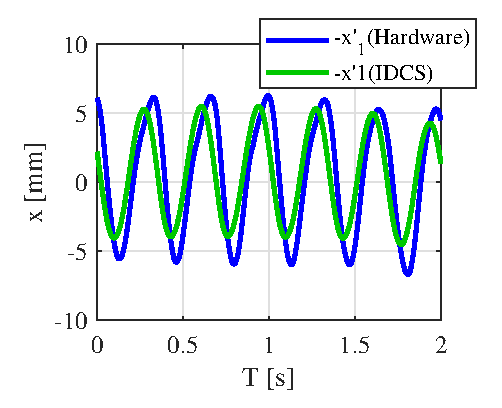
\includegraphics[height=30mm]{figure/idcs_nonlinear_5_3.eps}
      \end{center}
      \begin{center}
        \vspace{-4mm}
      \ (b)Comparison with Hardware model\
    \end{center}
  \end{minipage}
  \end{tabular}
  \caption{Result(nonlinear damper)}
    \label{fig:idcs_nonlinear}
\end{figure}

\section{結言}
本研究では,IDCSを用いたアクチュエータの制御手法のHILSシステムにおける再現性を評価した.解析モデルの計算結果と試験機の計測値を比較し,同様の挙動を示していることを確認した.また非線形特性を考慮したダンパモデルをIDCS制御系に組み込むことで,非線形性を考慮した制御を行えることを確認した.

\begin{thebibliography}{99}
\bibitem{hils}永井正夫,吉田秀久,Noomwongs Nuksit,横井隆,川眞田智,小林克宏,タイヤHILシミュレータによる車両運動性のの研究(第1報):タイヤHILシミュレータの開発,自動車記述会論文集,Vol.35,No.2,(2004),pp.147-152
\bibitem{2dof}社団法人 自動車技術会,自動車技術ハンドブック5設計(シャシ)編,社団法人 自動車技術会,(1990),p.25
\bibitem{method_idcs}青木 健悟,IDCSを用いた柔軟アームを有するロボットの振動制御,日本ロボット学会誌,Vol.31,No.10,(2010),pp.1001-1008
\end{thebibliography}

\end{document}
